\documentclass[a4paper,10pt]{article}

\usepackage{array}
\usepackage{bold-extra}
\usepackage{booktabs}
\usepackage{colortbl}
\usepackage{enumitem}
\usepackage[margin=10mm]{geometry}
\usepackage{graphicx}
  \graphicspath{{./Pictures/}}
\usepackage{hyperref}
\usepackage[utf8]{inputenc}
\usepackage{multirow}
\usepackage{ragged2e}
\usepackage{titlesec}
\usepackage{titling}
\usepackage{xcolor}
\usepackage[export]{adjustbox}

\definecolor{linkblue}{rgb}{0, 0.127, 0.4}
\definecolor{gralinski-violet}{rgb}{0.298, 0, 0.408}
\definecolor{solarized-violet}{rgb}{0.424, 0.443, 0.769}
\definecolor{dark-violet}{rgb}{0.424, 0.2, 0.769}
\definecolor{dark-gray}{rgb}{0.081, 0.081, 0.081}
\definecolor{tech-green}{RGB}{0, 127, 0}

\titleformat{\section}
{\color{dark-gray}\sffamily\scshape\huge\bfseries}
{}
{0em}
{}%[\titlerule]

\titleformat{\subsection}
{\bfseries\large}
{}
{0em}
{}

\titleformat{\subsubsection}[runin]
{\bfseries}
{}
{0em}
{}[ ---]

\titlespacing*{\section}{0pt}{0pt}{0pt}
\titlespacing*{\subsection}{0pt}{0pt}{3pt}

\setlength{\parindent}{0em}
\setlength{\parskip}{0em}
\setitemize{topsep=0pt,parsep=0pt,partopsep=0pt}

\newcolumntype{P}[1]{@{}>{\arraybackslash}p{#1}@{}}
\newcolumntype{M}[1]{@{}>{\centering\arraybackslash}m{#1}@{}}
\newcolumntype{B}[1]{@{}>{\arraybackslash}b{#1}@{}}

\hypersetup{%
  colorlinks=true,
  linkcolor=linkblue,
  urlcolor=linkblue,
}

\pagestyle{empty}

\begin{document}
\newcommand{\tech}[1]{\textbf{\texttt{\textcolor{tech-green}{#1}}}}
\renewcommand{\labelitemii}{$\circ$}

\raggedright{}

%%%%%%%%%%%%% Header %%%%%%%%%%%%%%%
\begin{table}
\begin{centering}

% Photo(25mm), header-name(95mm), contact-data(70mm).
% 190mm in total [210mm paper width minus 10mm page margin on both sides].
\arrayrulecolor{gralinski-violet}
\begin{tabular}{| M{25mm} | @{}M{115mm}@{} @{}M{50mm}@{} |}
  \hline
  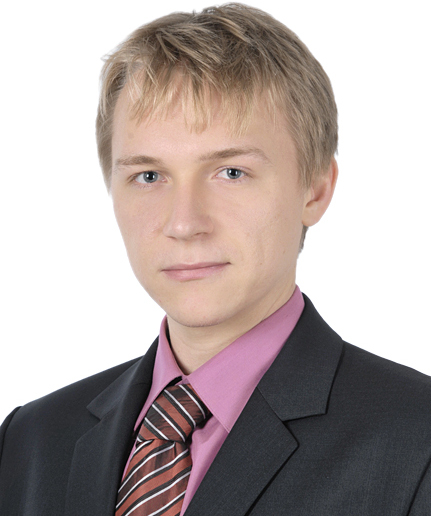
\includegraphics[width=25mm,height=31mm]{self}
  \vspace*{-5.5mm}
  &
  \begin{tabular}{M{115mm}}
    \vspace*{-10mm}
    \textbf{\Huge Adam Graliński} \\

    \vspace*{12pt}\textbf{\LARGE Software Engineer} \\
  \end{tabular}
  &
  \begin{tabular}{M{8mm} M{3mm} B{39mm}}
    \multirow{2}{*}{
\includegraphics[height=2em,keepaspectratio]{icon_location}} & &
    Majdańska 3/104, \\
    & & 04--088 Warsaw, Poland \\

    
\includegraphics[height=2em,keepaspectratio]{icon_email} & &
    \href{mailto:adam@gralin.ski}{adam@gralin.ski} \\

    
\includegraphics[height=2em,keepaspectratio]{icon_github} & &
    \href{https://github.com/agral}{github.com/agral}
  \end{tabular}

  \\ \hline
\end{tabular}
\end{centering}
\end{table}
%%%%%%%%%%%%% end-of-Header %%%%%%%%%%%%%%%

\section{Work experience}
\subsection{Self-employed, \textit{gralin.ski} \hfill 02.2020\,--\,present}
\begin{itemize}[leftmargin=15pt,itemsep=3pt]
  \item Ran a self-owned software consulting company
\end{itemize}

\vspace{18pt}
\subsection{Protocol Engineer, \textit{Samsung Electronics} \hfill 02.2020\,--\,present}
\begin{itemize}[leftmargin=15pt,itemsep=3pt]
  \item Maintenance and development work in \tech{C++} and \tech{Java} layers of Samsung's IMS framework
  \item Investigation of atypical problems in networked code (\tech{Wireshark})
  \item Development of automated C++ code review tool (\tech{python}, \tech{p4},
      \tech{cppcheck} \& \tech{clang})
\end{itemize}

\vspace{18pt}
\subsection{Senior C++ Developer, \textit{Huuuge Games} \hfill 03.2019\,--\,01.2020}
\begin{itemize}[leftmargin=15pt,itemsep=3pt]
  \item Huuuge Casino --- maintenance and development of a mobile social casino game
  \begin{itemize}
    \item AAA title; +2M monthly active users at that time
    \item Tech stack: \tech{C++}, \tech{Lua}
  \end{itemize}
  \item Huuuge Charms --- development of a novel feature for Huuuge Casino
  \begin{itemize}
    \item Tech stack: \tech{C++}, \tech{Lua}, \tech{flatbuf}, \tech{python}
  \end{itemize}
\end{itemize}

\vspace{18pt}
\subsection{C++ Developer, \textit{Huuuge Games} \hfill 08.2017\,--\,02.2019}
\begin{itemize}[leftmargin=15pt,itemsep=3pt]
  \item Development of Huuuge Stars --- a mobile social casino game made from scratch
        \hfill (01.2018\,--\,02.2019)
  \begin{itemize}
    \item Firsthand experience of a \textit{full development cycle} ---
          from scratch to a successful launch
    \item Fully remote development work
    \item Tech stack: \tech{C++}, \tech{Lua}, \tech{python}
  \end{itemize}
  \item Maintenance and development work for Huuuge Casino
  \begin{itemize}
    \item Tech stack: \tech{C++}, \tech{Lua}
  \end{itemize}
\end{itemize}

\vspace{18pt}
\subsection{Junior C++ Developer, \textit{Samsung Electronics} \hfill (11.2015\,--\,07.2017)}
\begin{itemize}[leftmargin=15pt,itemsep=3pt]
  \item {\bfseries Mobile solutions} \hfill{} (03.2017) \par
  Prepared and carried out a workshop for students of Warsaw University of Technology --- \par
  presented on WUT's career fair ``Inżynierskie Targi Pracy'' \par
  Slides (Polish):
  \href{https://github.com/agral/Lectures/blob/master/RozwiazaniaMobilne/RozwiazaniaMobilne.pdf}
  {github.com/agral/Lectures/blob/master/RozwiazaniaMobilne/RozwiazaniaMobilne.pdf}\par

  \item {\bfseries Samsung Academy R\&D} \hfill{} (02.2017\,--\,04.2017) \par
  Prepared and carried out a crash course for WUT students regarding creating\par
  Android applications with the use of \tech{Xamarin} library.\par
  The course is comprised of four workshops, each taking approximately 2.5\,--\,3 hours.\par
  Slides (Polish): \href{https://github.com/agral/Lectures/tree/master/AkademiaSamsung}
  {github.com/agral/Lectures/tree/master/AkademiaSamsung}\par


  \item {\bfseries Business trip to Seoul, South Korea} \hfill{} (10.2016) \par
  Assisted Microsoft with recording a promotional movie about Samsung/Microsoft cooperation.\par
  The movie has been aired live during \textit{Microsoft Connect(); 2016} conference.\par
  Video: \href{https://www.youtube.com/watch?v=m_fKcjhkY-0}{youtube.com/watch?v=m\_fKcjhkY-0}\par

  \item {\bfseries Business trip to Suwon, South Korea} \hfill{} (03.2016) \par
  Prepared a draft port of \tech{Xamarin} library to the Tizen platform in a team of three developers.\par
  The demo was very well received and resulted in a project grant in 2016--2017.\par

  \item Development work in the {\bfseries Tizen Platform Team} \hfill{} (11.2015)
  \begin{itemize}
    \item Porting the existing \tech{C API} collection to \tech{C\#} (\tech{Xamarin})
    \item Improving the \tech{JavaScript} API of \textit{Tizen OS}
    \item Improving the documentation (\tech{Doxygen})
  \end{itemize}
\end{itemize}

\pagebreak{}
\section{Education}
{\large\textbf{Master's degree \hfill (2014\,--\,2015)}} \par
\textit{Warsaw University of Technology, Faculty of Mechatronics}\par
Master's thesis: \textbf{Analysis of clustering algorithms}.\par

\vspace{12pt}
{\large\textbf{Bachelor's degree \hfill (2009\,--\,2014)}} \par
\textit{Warsaw University of Technology, Faculty of Mechatronics}\par
Thesis: \textbf{Design of impulse counter for flow meters (hardware\,+\,software)}.\par

\vspace*{24pt}
\begin{tabular}{ P{90.5mm} P{14mm} P{85.5mm} @{}m{0pt}@{} } % 190mm to use (210 in total)
\section{Skills}
\subsection{Programming languages:}
\begin{itemize}[leftmargin=15pt,itemsep=3pt]
  \item \tech{C++} (up to \tech{C++17} with bits of \tech{C++20})
  \item \tech{Java}
\end{itemize}

\vspace{9pt}
\subsection{Scripting languages:}
\begin{itemize}[leftmargin=15pt,itemsep=3pt]
  \item \tech{Python}
  \item \tech{Lua} (core + \tech{C API})
  \item Linux shell (\tech{sh}, \tech{bash}, \tech{zsh})
\end{itemize}

\vspace{9pt}
\subsection{Libraries:}
\begin{itemize}[leftmargin=15pt,itemsep=3pt]
  \item \tech{SDL2} (both fixed and functional pipelines)
  \item \tech{OpenGL},
  \item \tech{Catch2} (unit test library for C++)
  \item \tech{JUnit}, \tech{Mockito}, \tech{Robolectric} \par
        --- tech stack for Java unit tests
\end{itemize}

\vspace{9pt}
\subsection{Operating systems:}
\begin{itemize}[leftmargin=15pt,itemsep=3pt]
  \item \tech{Linux} (15+ years of experience)
  \item \tech{Windows} (18+ years of experience)
\end{itemize}

\vspace{9pt}
\subsection{Other:}
\begin{itemize}[leftmargin=15pt,itemsep=3pt]
  \item Version control: \tech{git}, \tech{Mercurial}, \tech{p4} (\tech{Perforce})
  \item Debugging and profiling tools:
  \begin{itemize}
    \item \tech{gdb}
    \item \tech{clang-tools}
    \item \tech{strace}
    \item google sanitizers (mostly \tech{TSAN} and \tech{ASAN})
  \end{itemize}
  \item In-depth knowledge of \tech{make} utility
  \item Practical experience with Atlassian toolset\par
    (\tech{JIRA}, \tech{Confluence}, etc.)\par
  \item Familiarity with \tech{agile} development methodologies,\par
    in particular \tech{Scrum} and \tech{kanban}
\end{itemize}

& &

\section{Languages proficiency}
\arrayrulecolor{black}
\hspace{7mm}\begin{tabular}{|c|c|c|c|}
\hline
\textbf{Language} & \textbf{Level} & \textbf{Written} & \textbf{Spoken} \\
\hline
Polish & native & Fluent & Fluent \\
\hline
English & C2 & Fluent & Fluent \\
\hline
German & B2 & Good & Fair \\
\hline
Italian & B1 & Good & Good \\
\hline
Korean & A1 & Beginner & Beginner \\
\hline
\end{tabular}

\vspace{24pt}
\section{Areas of personal interest}
\begin{itemize}[leftmargin=15pt,itemsep=3pt]
  \item Programming and scripting
  \item Automation in all its forms
  \item Rolling release linux distributions
  \item Sports: chess and long--distance running
  \item Travelling, especially to Asia
\end{itemize}
\\
\end{tabular}

\vspace{24pt}
{\small\textit{
I hereby give consent for~my~personal data included in~my~application to~be~processed
for~the~purposes of~the~recruitment process under the~Personal Data Protection Act as~of 29~August~1997,
consolidated text: Journal of~Laws 2016, item 922 as~amended.}\par
}
\end{document}
